%%=============================================================================
%% Conclusie
%%=============================================================================

\chapter{Conclusie}
\label{ch:conclusie}

%% TODO: Trek een duidelijke conclusie, in de vorm van een antwoord op de
%% onderzoeksvra(a)g(en). Wat was jouw bijdrage aan het onderzoeksdomein en
%% hoe biedt dit meerwaarde aan het vakgebied/doelgroep? Reflecteer kritisch
%% over het resultaat. Had je deze uitkomst verwacht? Zijn er zaken die nog
%% niet duidelijk zijn? Heeft het onderzoek geleid tot nieuwe vragen die
%% uitnodigen tot verder onderzoek?

\section{Inleiding}
Redux is een framework dat nog maar 3 jaar bestaat. Er is wel al veel documentatie beschikbaar en veel problemen zijn reeds ontdekt en opgelost, maar zeker niet alles staat beschreven. 

Bijvoorbeeld hoe 2 React-Redux projecten met elkaar kunnen interageren staat nergens beschreven. Omdat hier geen best practices vermeld werden, is de keuze gemaakt om via npm packages te werken. Op deze manier kan het ene project snel geïntegreerd worden in het andere. 

Het was echter niet voldoende om deze package gewoon te installeren. Wanneer dan een component werd aangeroepen zou de state niet volledig zijn. De state bevat dan enkel objecten van het hoofdproject en niet van het geïntegreerde project. Om deze reden moeten de reducers geëxporteerd worden uit het geïntegreerde project. 

\section{Performantie}
Zoals eerder vermeld was de oplossing om deze reducers in een object te steken en dit te exporteren. Het grootste probleem hierbij is dat veranderingen in het project dat geïntegreerd moet worden grote gevolgen kan hebben. Dit werd ondervonden door het open source project van Scratch. Na een update van Scratch uit en de bijhorende update om de package up-to-date te houden werkte deze niet meer. Dit kwam door een verandering in de structuur van de reducers, waardoor het niet meer de juiste reducers waren die geëxporteerd werden. Dit zorgt er dus voor dat er zeer aandachtig moet gebleven worden bij updates. Om deze reden zou er nood zijn aan een methode uncombineReducers of een alternatief waardoor er enkel met de root reducer rekening zou gehouden moeten worden. Dan zouden externe updates geen grote impact meer hebben en kan deze snel terug geïntegreerd worden.

Deze methode is niet optimaal, aangezien er heel wat onderhoudswerk bij komt kijken om de package up-to-date te houden. Een bijkomend probleem is dat met deze methode ook alle dependencies moeten overgenomen worden alsook de webpack configuraties. 

Deze methode wordt al een heel stuk performanter door het te integreren project te combineren in webpack, op deze manier is het niet meer nodig om alle dependencies toe te voegen aan het hoofdproject en wordt de package voor de webpack configuraties overbodig. 

Zoals eerder gezegd is deze methode afhankelijk van de veranderingen in het te integreren project. Als hier quasi geen veranderingen in moeten gebeuren zal dit geen grote impact hebben, als er constant veranderingen in gebeuren dan zal deze methode niet meer optimaal zijn. 

\section{Complexiteit}
Er zijn een aantal objectieve maatstaven die ontwikkeld zijn om de complexiteit van software te meten. In grote lijnen kan men deze maatstaven verdelen in maten voor complexiteit die zijn gerelateerd aan de omvang van een software-programma, en in maten voor complexiteit die zijn gerelateerd aan de structuur van zo'n programma. De simpelste maat voor de omvang is het aantal regels programmacode: hoe meer regels, hoe groter de complexiteit. Een ernstig nadeel van deze simpele metriek is dat men het verschil in uitdrukkingskracht van de verschillende programmeertalen volledig verwaarloost.

Men maakt ook geen onderscheid naar soorten regels code. Er zijn echter eenvoudige regels code en er zijn complex samengestelde regels programmacode. Om hieraan tegemoet te komen, heeft Halstead een meer verfijnde metriek ontwikkeld. In zijn theorie is de complexiteit en de daarmee samenhangende programmeerinspanning afhankelijk van de omvang van een programma en van het niveau van structurering. Hoe groter de omvang, hoe hoger de programmeerinspanning. Hoe hoger (compacter) het niveau van structurering, hoe lager de inspanning. Zowel omvang als niveau van structurering zijn functies van het aantal verschillende operatoren en operanden in een programma.
\autocite{complexiteit01}





\begin{figure}
	\begin{center}
		\caption{De formule van Halstead uitgelegd. Verkregen van \textcite{halstead}}
		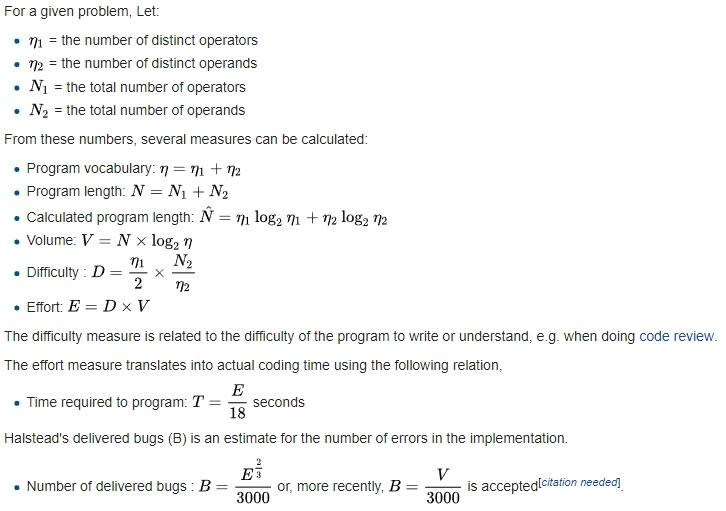
\includegraphics[width=16cm]{img/halstead}\\[0.5cm]
	\end{center}
\end{figure}


Men kan nu deze metriek toepassen op het voorbeeld met de gemaakte package in deze studie. n1 staat voor het aantal verschillende operatoren, n2 staat voor het verschillende aantal operanden, N1 is het aantal operatoren en N2 is het aantal operanden. Met deze nummers kunnen een aantal metingen berekend worden:
\begin{itemize}
	\item Vocabulair van het programma: n = $n_1$ + $n_2$ = 3 + 23 = 27.
	\item Lengte van het programma: N = $N_1$ + $N_2$ = 27 + 43 = 70.
	\item Berekende lengte van het programma: $N_3$ = $n_1$ $log_{2}(n_1)$ + $n_2$ $log_{2}(n_2)$ = 4,7549 +  104,0419 = 108,7968.
	\item Volume: V = N * $log_{2}(n)$ = 70 * 4,7549 = 332,8422.
	\item Moeilijkheid: D = ($n_1$/2) * ($N_2/n_2$) = 1,5 * 1,8696 = 2,8043.
	\item Inspanning: E = D * V = 2,8043 * 332,8422 = 933,3894.
\end{itemize}
De meeteenheid inspanning kan vertaald worden naar codeertijd aan de hand van de volgende relatie: de tijd T = E/18 = 51,8550 seconden.
Halstead kan ook een schatting geven van het aantal errors die in de implementatie zitten door naar het aantal geleverde bugs te kijken: B = E\textsuperscript{2/3}/3000 = 0,1245.

Deze metriek werd toegepast op het exporteren van de reducers in de gepubliceerde package en de code die nodig is om alle reducers opnieuw te importeren in een hoofdproject. Er kan geconcludeerd worden dat het een snelle codeertijd heeft dat gepaard gaat met een laag aantal geleverde bugs.

Een andere manier om de complexiteit van software te meten is via de cyclomatische complexiteit. Deze metriek is een quantitatieve meting van het aantal lineair onafhankelijke paden in de code en werd ontwikkeld door McCabe. 
De cyclomatische complexiteit wordt gedefinieerd als M = E - N + 2P.\newline
Waarbij: 
\begin{itemize}
	\item E = het aantal randen, verbindingen in een diagram
	\item N = het aantal knooppunten in een diagram
	\item P = het aantal geconnecteerde componenten
\end{itemize}
\autocite{cyclomatic}

In dit geval gaat het om een lineaire structuur zoals gezien kan worden in de figuur. De geëxporteerde package bevat 23 verbindingen, 24 knooppunten en 1 geconnecteerde component. Hiermee kan de cyclomatische complexiteit bepaald worden door M = 23 - 24 + 2 = 1. Volgende figuur verkregen uit \textcite{complexitynumbers} geeft een overzicht weer van de complexiteit waarde en zijn overeenkomstige betekenis. 

Hieruit kan afgelezen worden dat een nummer hoger dan 40 niet getest kan worden en een hoge kost en inspanning heeft. Een waarde tussen de 20 en 40 wordt aanzien als heel complexe code met lage test mogelijkheden en eveneens een hoge kost en inspanning. Een complexiteitswaarde tussen de 10 en 20 duidt op complexe code met gemiddelde testbaarheid, kost en inspanning. Een waarde tussen de 1 en 10 betekent dat de code goed gestructureerd en geschreven is, met een hoge testbaarheid en een lage kost en inspanning. Aangezien de berekende cyclomatische complexiteit 1 bedraagt, kan de conclusie getrokken worden dat de code gestructureerd is, een lage kost en inspanning heeft en makkelijk getest kan worden.


Een derde manier om de complexiteit van een programma te meten is aan de hand van een maintainability index. De maintainability index is een metriek  die meet hoe onderhoudbaar de source code is. Deze index wordt berekend door een aantal factoren, de formule maakt gebruik van lines of code, cyclomatic complexity en Halstead volume. Deze metriek wordt onder andere gebruikt in verschillende geautomatiseerde software tools in Visual Studio, daar gebruikt het een schaal van 0 tot 100.
Om deze index te meten wordt gebruik gemaakt van de formule: \newline MI = 171 - 5,2 * ln(V) - 0,23 * (G) - 16,2 * ln(LOC) \\
Hierbij horend: 
\begin{itemize}
	\item V = Halstead volume
	\item G = Cyclomatische complexiteit
	\item LOC = het aantal lines of code
\end{itemize}
\autocite{maintainability01}\newline\newline
Wanneer deze formule toegepast wordt op het voorbeeld van de npm package met de geëxporteerde reducers en de code die nodig is in het hoofdproject om deze reducers opnieuw te importeren, dan krijgen we: \newline
MI = 171 - 5,2 * ln(332,8422) - 0,23*1 - 16,2*ln(43) = 171 - 30,1999 - 0,23 - 60.9314 = 79,6387. \newline
Volgens \textcite{maintainability02} heeft een programma met hoge onderhoudbaarheid een waarde tussen de 20 en 100. Een waarde tussen 10 en 19 wil zeggen dat de code een gemiddelde onderhoudbaarheid heeft en een waarde tussen de 0 en 9 duidt op een slechte, lage onderhoudbaarheid van het programma. In dit voorbeeld is de maintainability index 79,6387, dit wil zeggen dat er op basis van deze index kan afgeleid worden dat het programma een hoge, goeie onderhoudbaarheid heeft. Men kan echter geen conclusie maken op basis van de maintainability index alleen. Dit komt omdat deze index een bewerking uitvoert met 3 metrieken. Onder deze metrieken bevinden zich de lines of code en de cyclomatische complexiteit. Om deze goeie onderhoudbaarheid te testen kan er gekeken worden naar de andere metingen die zijn uitgevoerd.  Halstead had een goeie waarde met een lage codeertijd en een laag aantal geleverde bugs. De cyclomatic complexity had uiteraard ook een goeie waarde aangezien het gaat om een volledig lineaire structuur (M = 1). Deze combinatie van metrieken zorgt ervoor dat er finaal geconcludeerd kan worden dat het programma een hoge onderhoudbaarheid heeft met een lage complexiteit. 

\section{Eindconclusie}
Dit onderzoek is nog niet klaar, de basis is wel gelegd om verder onderzoek te doen naar een methode om de root reducers van beide projecten met elkaar te combineren zonder dat daar veel extra onderhoud aan te pas komt. Als uitkomst was wel verwacht dat er een soort uncombineReducers zou gemaakt worden, helaas was dit niet mogelijk door de implementatie van deze functie. Er is wel een alternatief gevonden om toch het probleem op te lossen. 

Achteraf gezien bleek het een goede keuze om voor het Scratch open source project te kiezen. Dit is een project dat nog steeds in development is en dat nu overschakelt op JavaScript, waardoor het zeer interessant wordt om dit te kunnen integreren in een eigen applicatie.   

Dit is een belangrijk onderzoek omdat er nog geen soortgelijke onderzoeken zijn gedaan of gedocumenteerd werden.
Er zijn een aantal statistieken gevonden die duidelijk maken dat het een probleemstelling is die uitnodigt tot verder onderzoek. De npm package die de reducer exports verzorgde is opgericht eind februari. Dan werd gezocht naar hoe het mogelijk wordt om dit project snel integreerbaar te maken, waar tot een tijdelijke oplossing is gekomen begin maart. Deze package werd sinds dan ruim 7000 keer gedownload (figuur 3.4) met piekmomenten van 2168 downloads per week (figuur 3.3) en 946 downloads per dag (figuur 3.2) in maart. Door tijdsgebrek was het echter onmogelijk om deze package constant up-to-date te houden. Eind maart kan er nog een update gezien worden door het stijgende aantal downloads, wat duidt op het feit dat er wel vraag naar is.


Als conclusie kan ook gesteld worden dat het momenteel niet mogelijk is om twee root reducers met elkaar te combineren via de functie combineReducers waarbij de functionaliteit van beide root reducers behouden wordt. Hiernaast kan wel gezegd worden dat het mogelijk is om de functionaliteit van twee React-Redux projecten te combineren door een export te maken van de reducers die de functionaliteit ondersteunen die geïntegreerd zou moeten worden in het project. Deze export moet wel beschikbaar gemaakt worden op npm om daarna de mogelijk te bieden om deze als dependency te installeren. Het is ook mogelijk om het volledige project te bundelen via webpack eens er geen veranderingen meer nodig zijn. Na objectief onderzoek blijkt dit een weinig complexe en goed onderhoudbare oplossing. Toch kan er nog altijd onderzoek gebeuren naar een methode om twee gecombineerde reducers met elkaar te combineren. 


\newpage

\begin{figure}
	\begin{center}
		\caption{Downloads per dag van de geëxporteerde package. Verkregen van \textcite{npm}}
		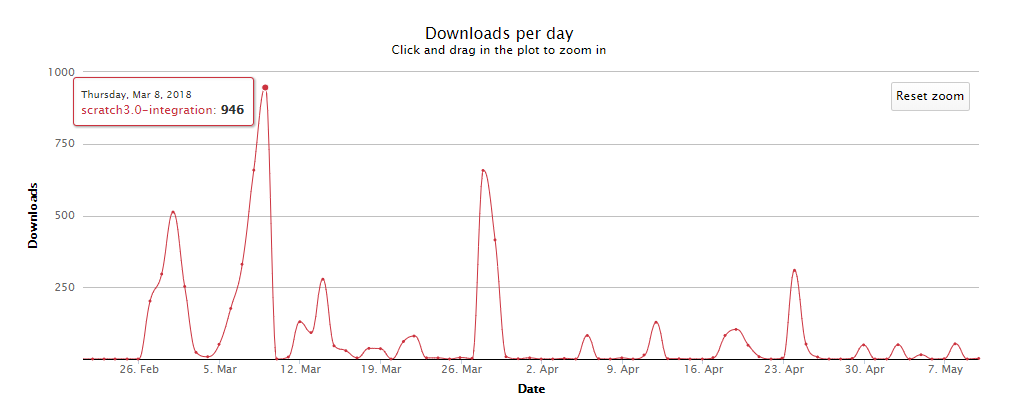
\includegraphics[width=16cm]{img/package-downloads-day}\\[0.5cm]
	\end{center}
\end{figure}
\begin{figure}
	\begin{center}
		\caption{Downloads per week van de geëxporteerde package. Verkregen van \textcite{npm}}
		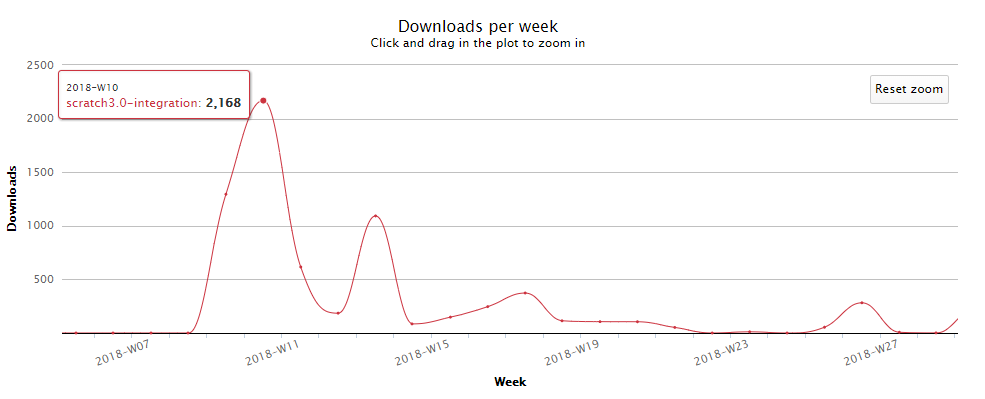
\includegraphics[width=16cm]{img/package-downloads-week}\\[0.5cm]
	\end{center}
\end{figure}
\begin{figure}
	\begin{center}
		\caption{Totale downloads van de geëxporteerde package. Verkregen van \textcite{npm}}
		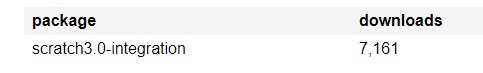
\includegraphics[width=16cm]{img/package-total-downloads}\\[0.5cm]
	\end{center}
\end{figure}